%Part of/Parte di https://github.com/f-dinucci/appuntiMeccanicaFluidi/
%License/Licenza Creative Commons Attribution-ShareAlike 4.0 International (CC BY-SA 4.0) - attribution/attribuzione Francesco Di Nucci
%See also/Vedere anche https://creativecommons.org/licenses/by-sa/4.0/ and/e https://creativecommons.org/licenses/by-sa/4.0/legalcode
%
\section{Proprietà locali conservate}
Nello studio dei fluidi vi sono alcune proprietà di interesse.
Si definiscono \textit{proprietà conservate} quelle proprietà che sono costanti se non vi sono forze esterne al sistema in analisi: esse sono massa, quantità di moto ed energia.
\subsection{Proprietà conservate nei solidi}
\subsubsection{Quantità di moto}
Nei solidi la quantità di moto varia nel tempo solamente per l'azione di forze esterne al sistema (esercitate cioè da qualcosa diverso dagli oggetti nel sistema):
%
	\begin{equation*}
		\dv{t} (m_1 \uline{v}_1 + m_2 \uline{v}_2) = \uline{F}_{ext}
	\end{equation*}
%
	\begin{figure}[H]
		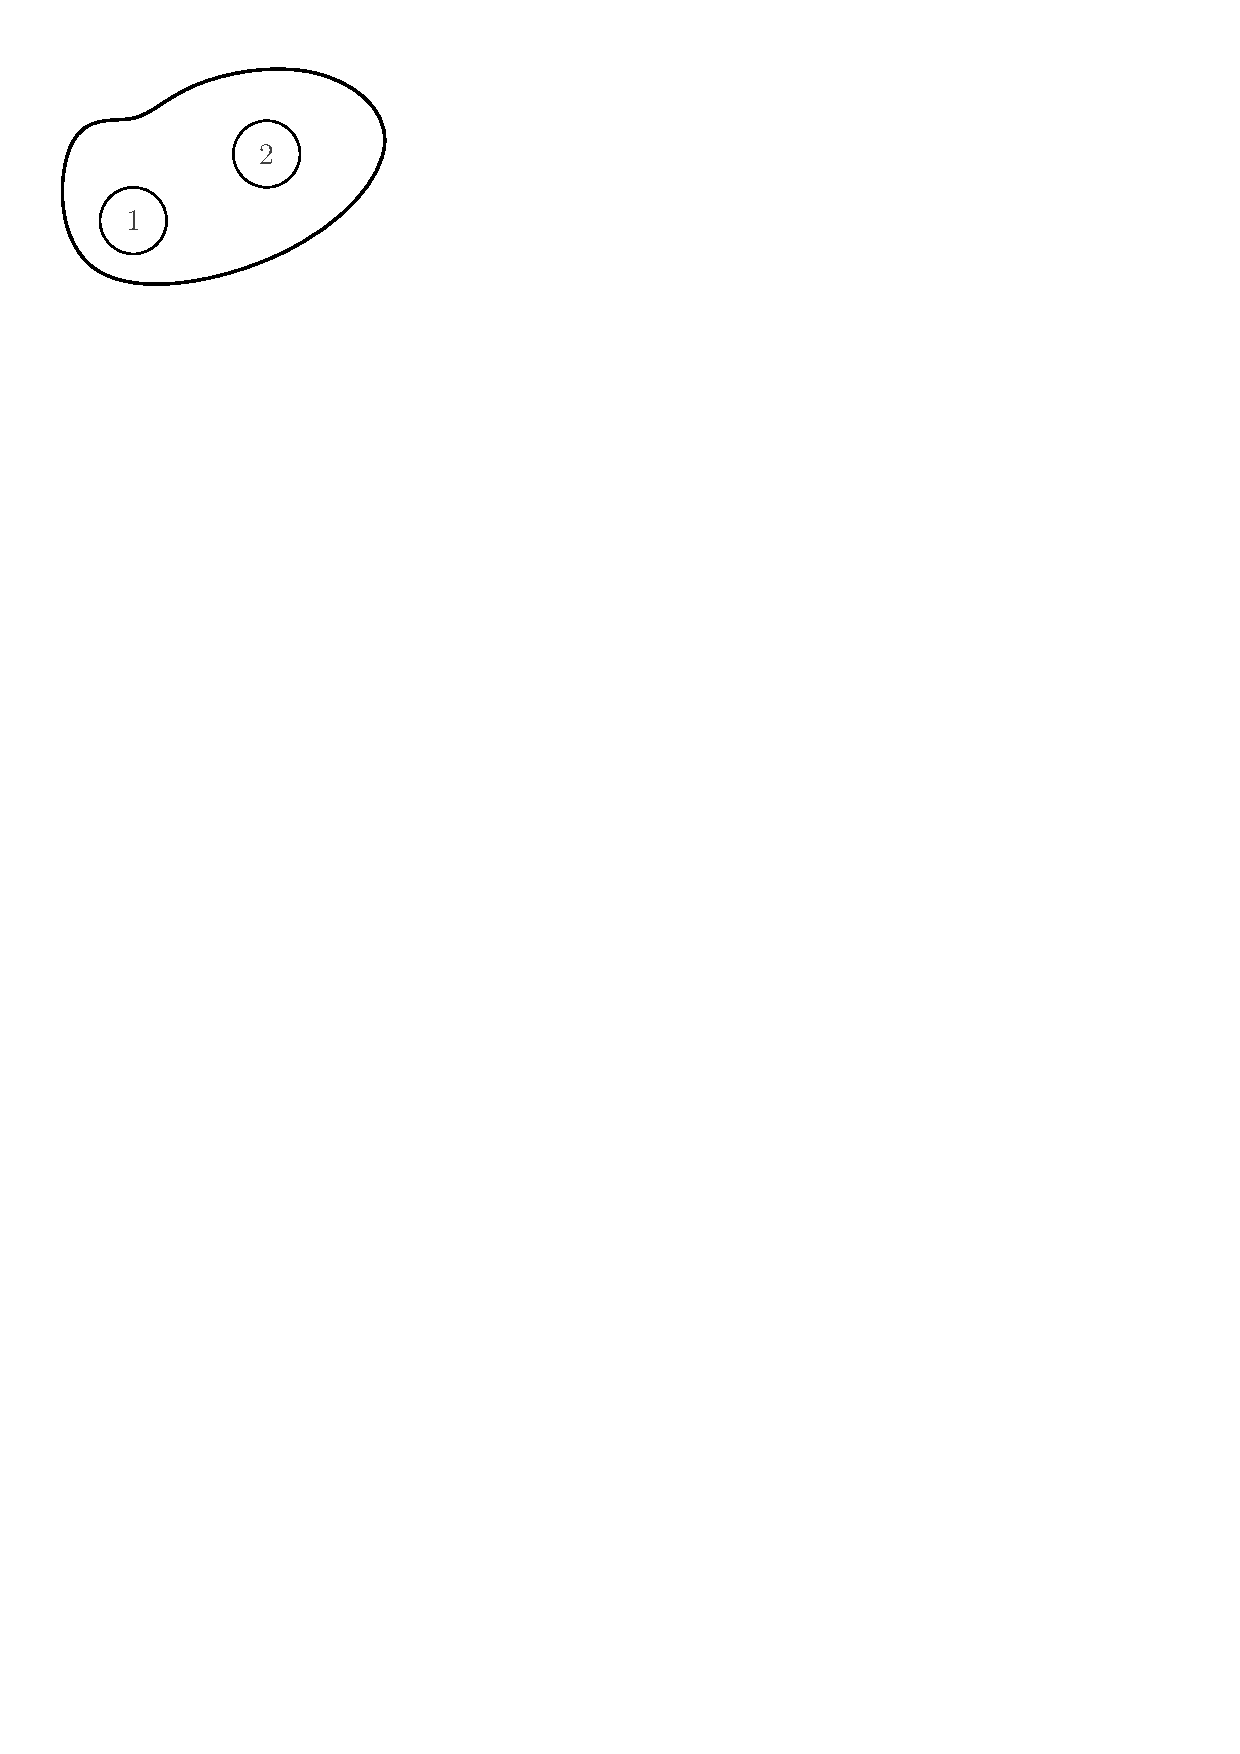
\includegraphics[scale=0.8]{./1.2 Proprietà locali conservate/1.2-1}
		\centering
		\caption{Si prendano ad esempio due particelle di un solido}
	\end{figure}
%
Cioè la quantità di moto varia nel tempo solamente se la risultante delle forze esterne è diversa da zero, nel caso in cui $\uline{F}_{ext} = \uline{0}$ (ad esempio per un sistema chiuso) invece è costante.
\subsubsection{Energia}
Il ragionamento è simile per l'energia, che in un sistema chiuso varia solamente se il lavoro delle forze esterne non è nullo, ($L_{ext} \neq 0$):
%
	\begin{equation*}
		\dv{t} (E_1 + E_2) = L_{ext}
	\end{equation*}
%
\subsubsection{Massa}
Anche la massa \textit{totale} del sistema è costante:
%
	\begin{equation*}
		\dv{t} (M_1 + M_2) = 0
	\end{equation*}
%
Da notare che si tratta di massa \textit{totale} del sistema, la massa dei singoli oggetti può anche cambiare (ad esempio a causa di reazioni chimiche).
%
\subsection{Proprietà conservate nei fluidi}
Si dimostra che anche in un volume \textit{V}  di fluido quantità di moto, energia e massa sono grandezze conservate: per portare i risultati di cui prima nella meccanica del continuo si divide il volume di fluido in \textit{n} parti infinitesime, ognuna con la sua massa, effettuando poi una somma al limite tramite integrale. La legge di conservazione di una quantità qualsiasi assumerà quindi una forma del tipo:
%
	\begin{equation*}
		X = \int_V f \dd{V}	
	\end{equation*}
%
\subsection*{Bibliografia 1.2}
\cite[Cap.\ 1.3]{PnueliGutfinger}
